\documentclass[Bachelorarbeit.tex]{subfiles}
\begin{document}
\chapter{Evaluation}
\label{chap:evalutation}

Nachdem der Prototyp implementiert wurde, stellt sich die Frage, ob die Entwicklung und Ausarbeitung einen Mehrwert für Anwender\_innen darstellt. 
Dies soll nun mittels der Evaluation geklärt werden.
Für diesen Zweck sowie etwaige Schwachstellen aufzufinden soll der Prototyp im Rahmen einer Usability-Analyse auf Effektivität, Effizienz und Zufriedenstellung \cite[vgl.][Abs.: 3]{Iso9241_11} untersucht werden (siehe Abschnitt: \nameref{Methodik}).\\
\\
Der Ablauf der Usability Evaluation sieht dabei wie folgt aus.
Der Zweck sowie die zu untersuchenden Kriterien (siehe Absatz: \nameref{Usability}) erläutert.
Darauf folgt die Festlegung und Beschreibung der Verfahren welche zum Messen der Kriterien angewandt werden.
Im Abschnitt \nameref{Stichproben} wird der Rahmen für die Tests sowie die Auswahl der Proband\_innen festgelegt. 
Basierend auf den definierten Verfahren, wird im Abschnitt \nameref{Aufgabenstellung} die Erstellung und Begründung für die Auswahl des Testmaterials dargelegt, welches in der finalen Version auch im Anhang zu finden ist (siehe Anhang: \ref{anhangTestmaterial} - \nameref{anhangTestmaterial}).
Die anschließende Dokumentation sowie die Ergebnisse der Durchführung werden im Abschnitt \nameref{Ergebnisse} aufgezeigt.
Abschließend findet eine \nameref{InterpretationDiskussion} auf der Basis der Ergebnisse statt die unter anderen die Evaluation der \nameref{Hypothese} klärt.

\section{Methodik}
\label{Methodik}

Da die Interviews im Vorfeld ergeben haben, dass jede befragte Person einen unterschiedlichen Ablauf sowie unterschiedliche Werkzeuge bei der Planung der Außendienstrouten einsetzt, hilft ein vergleichender Test zwischen Status Quo und Prototyp an dieser Stelle nicht weiter.
Aus diesem Grund liegt es nahe einen klaren Schnitt zu den diversen alten Systemen zu ziehen und eine Formative Usability Evaluation\footnote{Bei der Formativen Evaluation wird anhand definierter Kriterien untersucht ob der Entwurf weiter optimiert werden kann. (vgl. \cite{Burmester}, S. 343)} nach den Kriterien der ISO 9241 durchzuführen.
Dafür soll der Prototyp auf die folgende Hypothesen hin mit Benutzerorientierten Methoden\footnote{Dabei liegt der Fokus bei den Tests auf definierten Anwender\_innen-Gruppen. (vgl. \cite{Burmester}, S. 343)} untersucht werden.


\subsection{Hypothese}
\label{Hypothese}

Der Prototyp unterstützt die potentiellen Pery-Anwender\_innen messbar in den Bereichen Effektivität, Effizienz und Zufriedenstellung bei der Planung von Außendiensteinsätzen (Die Begriffe Effektivität, Effizienz und Zufriedenstellung beziehen sich auf die Definition nach der Norm EN ISO 9241-11, \cite[vgl.][Abs.: 3]{Iso9241_11}).


\subsection{Exkurs Usability}  
\label{Usability}
Durch den sinnvollen Einsatz von Usability-Maßnahmen in der Entwicklung lässt sich die Qualität eines Produktes spürbar erhöhen.
Neben der Steigerung der Produktivität sowie der Zufriedenheit der Anwender\_innen werden laut Burmester auch die Einschulungszeiten bei dem Produkt deutlich verringert (\cite[vgl.][352f]{Burmester}).\\
\\
Im deutschsprachigen Raum werden die zwei Begriffe Gebrauchstauglichkeit und Softwareergonomie in Kontext mit Usability gesetzt.
Dabei gilt es allerdings zu beachten, dass der Begriff Softwareergonomie über den Umfang der Gebrauchstauglichkeit hinausreicht wie Beispielsweise Korrektheitsergonomie und Funktionsergonomie
(\cite[vgl.][420]{Niegemann2008})\\
\\
Innerhalb dieser Arbeit wird der Begriff Usability im Kontext der Gebrauchstauglichkeit verwendet die wie folgt in der ISO 9241 definiert wurde (\cite[siehe:][Abs.: 3.1 Gebrauchstauglichkeit]{Iso9241_11}):

\begin{quote}
	"\textit{Das Ausmaß, in dem ein Produkt durch bestimmte Benutzer in einem bestimmten Nutzungskontext genutzt werden kann, um bestimmte Ziele effektiv, effizient und zufriedenstellend zu erreichen.}" 
\end{quote}

Laut dieser Definition ergibt somit die Usability-Evaluation (Gebrauchstauglichkeit) inwiefern der Prototyp (Produkt) die Anwender\_innen bei der Planung der Außendienstroute (Nutzungskontext) unterstützt.

\paragraph{Effektiv}
Die Effektivität beschreibt ob und wie exakt es möglich ist die gestellte Aufgabe innerhalb des Nutzungskontext zu lösen.
Für diesen Zweck muss betrachtet werden inwiefern die Funktionalität des Prototyps die Anwender\_innen bei dem erreichen des Ziels, innerhalb eines definierte Szenarios unterstützt (vgl. \cite{Iso9241_11}, S. 4 sowie \cite{Burmester}, S. 325). \\
\\
Ein negativ Beispiel anhand des Prototyps könnte wie folgt aussehen.
Die Aufgabenstellung verlangt, dass alle Kunden ausgewählt werden sollen die innerhalb des letzten 24 Stunden Bestellungen aufgegeben haben. 
Wenn der Prototyp allerdings nur die Möglichkeit anbietet Kunden anzuzeigen die innerhalb der letzten Woche bestellt haben kann das Ziel nicht erfüllt werden und ist somit nicht Effizient.

\paragraph{Effizient}
Die Effizienz beschreibt wie viel Aufwand für die Lösung der Aufgabe innerhalb des Nutzungskontext nötig ist. 
Dabei trägt neben der Funktionalität das \ac{UI} (beispielsweise die Übersichtlichkeit und Erforschbarkeit) des Prototypen eine tragende Rolle inwiefern die Anwender\_innen zügig und sicher die Aufgabe bewältigen können (vgl. \cite{Iso9241_11}, S. 4 sowie \cite{Niegemann2008}, S. 421f).\\
\\
Ein Beispiel anhand des Prototypen könnte wie folgt aussehen.
Die Aufgabenstellung gibt an das ein Partnerkontakt besucht werden soll. Zusätzlich soll evaluiert werden welche weiteren Partnerkontakte sich in der nähe (ca. 1 Km) befinden, dabei sollen auch Stadtgrenzen übergreifend Adressen berücksichtigt werden (siehe Abb.: \ref{fig:HarteGrenzen} in Kapitel \nameref{chap:entwicklung} für die Visualisierung des Problems).
Durch die Bereitstellung einer Kartenansicht kann in diesem Fall die Effizient deutlich gesteigert werden. 

\paragraph{Zufriedenstellend}
Die Zufriedenstellung ist gegeben wenn die Anwender\_innen nicht durch das System behindert werden und eine positive Meinung über das Produkt haben. (vgl. \cite{Burmester}, S. 326)
Dies ist unter anderem zu erreichen in dem die Erwartungshaltung der Anwender\_innen gegenüber dem Produkt (Funktionsumfang und \ac{UI}) erfüllt werden.
Des weiteren ist es zu vermeiden  die Anwender\_innen durch aufwendige Dialoge oder einen unstrukturierten Aufbau des \ac{UI}'s in ihren Arbeitsfluss zu Beeinträchtigen.
Dadurch stellt sich laut Niegemann eine subjektiv positive Haltung ein was wiederum die Grundlage für die Akzeptanz des Produktes darstellt (vgl. \cite{Iso9241_11}, S. 4 sowie \cite{Niegemann2008}, S. 422).\\
\\
Ein mögliches negativ Beispiel könnte das unerwartet Verhalten der Applikation sein.
In der Kartendarstellung des Prototypen werden verschiedene Adressen auf der Karte dargestellt, dabei handelt es sich zum einen um Kunden und zum anderen um Lieferanten. 
Wenn sich das Verhalten, bei dem Klick auf einen der Marker, für die Anwender\_innen auf eine voneinander unlogische Weise unterscheidet\footnote{Beispielsweise wird bei einem Klick auf einen Kunden ein Popup  und bei einem Lieferanten eine vollständige Detailansicht (welche die Kartenansicht ersetzt) geöffnet.} ist dies irritiert und hemmt die Anwender\_innen in ihren Arbeitsfluss.
Was zur wiederum zur Folge hat, das sich keine Zufriedenstellung einstellt und auch keine Akzeptanz gegenüber dem Produkt etabliert.


\paragraph{Nutzungskontext}

Ein weiterer wichtiger Punkt stellt der Nutzungskontext da und definiert den Rahmen in dem die Evaluation durchgeführt wird.
Anhand der ISO 9241 wird der Nutzungskontext wie folgt definiert (siehe \cite{Iso9241_11}, S. 4). 

\begin{quote}
\textit{"Die Benutzer, die Arbeitsaufgaben, Arbeitsmittel (Hardware, Software und Materialien) sowie die physische und soziale Umgebung, in der das Produkt genutzt wird."}
\end{quote} 

Somit wird anhand der Tests nicht eine allgemeine Gebrauchstüchtigkeit evaluiert, sondern ausschließlich die Gebrauchstüchtigkeit des Produktes für den jeweils definierten Nutzungskontext.

\subsection{Verfahren}
\label{Verfahren}
Um den Prototypen auf die Gebrauchsfähigkeit (siehe Absatz \nameref{Usability}) hin zu untersuchen, muss geklärt werden, wie die Kriterien Effektivität, Effizienz und Zufriedenstellung sinnvoll gemessen werden können. 
Für diesen Zweck werden an dieser Stelle die Verfahren definiert und erläutert, welche die Grundlage für die Datenerhebung darstellen.

\paragraph{Effektiv}
In erster Linie soll die Effektivität mit Hilfe des \nameref{Eyetracking}-Verfahren ermittelt werden.
Dabei wird in der Auswertung analysiert, ob die Testpersonen die gestellten Aufgaben mithilfe des Prototypen bewältigen konnten.
Zu dem \nameref{Eyetracking} ergänzend erfolgt eine subjektive Einschätzung anhand eines geführten \nameref{FragebogenEvaluation}s. 

\paragraph{Effizient}
Auch im Bereich der Effizienz basiert die Analyse verstärkt auf dem \nameref{Eyetracking}-Verfahren welches durch die Erhebung des \nameref{FragebogenEvaluation}s um die persönliche Meinung sowie Anmerkungen der Testpersonen erweitert wird.
Mit Hilfe des \nameref{Eyetracking}s soll analysiert werden ob sich die Bearbeitungsdauer der einzelnen Testfälle linear zu deren Schwierigkeitsgrad verhält. 

\paragraph{Zufriedenstellend}
Im Gegensatz zu der Effektiv und der Effizient verhält sich Messung der Zufriedenstellung etwas subjektiver da es kein objektives Messkriterium gibt welches evaluiert werden kann.
Laut Burmester ist dieses Ziel erreicht wenn  die Testpersonen durch den Prototypen nicht behindert werden und sich bei ihnen ein positives Gefühl einstellt (vgl. \cite{Burmester}, S. 326). 
Für die Analyse dieser Dimension wird zum einen Fragen im rahmen des Fragebogens gestellt und zum anderen Bemerkungen der Testpersonen während des \nameref{Eyetracking}-Tests aufgezeichnet.
Im Anschluss an den Fragebogen soll geklärt werden, ob diese Bemerkungen einer subjektiv positiven- oder negativen Einstellung zuzuordnen sind.

\paragraph{Nutzungskontext}
\label{Nutzungskontext}
Die Testperson, welche eine natürliche Person mit Interesse an der Software Pery ist, soll selbständig mit Hilfe des entwickelten Prototypen (Arbeitstitel Pery Dispatch) verschiedener Szenarios der   Außendienstplanung durchführen. 
Für diesen Zweck findet im Vorfeld eine kurze mündlichen Einführung durch eine betreuende Person (Perfany Mitarbeiter\_in und/oder verantwortliche Person im Unternehmen) statt.
Bei Problemen, welche die Effektivität gefährden kann eine mündliche Nachfrage (telefonischer Support oder direktes Gespräch) mit einer betreuenden Person erfolgen. 
Für die Bearbeitung stehen der Person ein geeigneter Computerarbeitsplatz (PC, Monitor sowie benötigte Peripheriegeräte), ein funktionstüchtiger und aktueller Internetbrowser (Mozilla Firefox oder Google Chrome) sowie eine funktionierende Internetverbindung zur Verfügung.


\subsubsection{Eyetracking}
\label{Eyetracking}

Eyetracking gibt uns die Möglichkeit Objektive Daten über das Verhalten der Anwender im Kontext der Interaktion mit dem System zu erhalten.
Während in Tests ohne Eyetracking meist Aufzeichnung von klassischen Benutzeraktionen wie beispielsweise Eingabegeräte (Maus und Tastatur) sowie Kameraaufzeichnungen des Bildschirms und der Proband\_innen erfasst werden, können durch Eyetracking zusätzliche Informationen wie das Verhalten evaluiert werden.
Bei diesen zusätzlichen Messdaten geben Ausschluss darüber ob und in welcher Reihenfolge Informationen des \ac{UI}'s durch die Proband\_innen wahrgenommen wurden. (vgl. \cite{Niegemann2008}, S. 439ff und \cite{Burmester}, S. 347ff)\\
\\
Um die Technologie zu verstehen muss man wissen das unser Auge mit zwei Zuständen Fixation und Sukkaden arbeitet.
Bei der Fixation blickt das Auge auf einen Punkt und es findet die Informationsverarbeitung statt. 
Während bei der Sukkade der Blick zur nächsten Informationsquelle springt bei der Anschließend wieder eine Fixation stattfindet. (vgl. \cite{Burmester}, S. 347f)\\
\\
Durch diesen Effekt kann mit Hilfe des Eyetrackingssystems eine Blickabfolge erstellt und ausgewertet werden (siehe Abb.: \ref{fig:Eyetracking}-1).
Zusätzlich zu der Blickabfolge können auch sogenannte Heatmaps erstellt werden, diese visualisieren wie lang auf einen bestimmten Bereich des Monitors geblickt wurde (siehe Abb.: \ref{fig:Eyetracking}-2).
Mithilfe der Auswertung von diesen beiden Analysen erhalten wir schlussendlich Informationen darüber welche Inhalte wie schnell und sicher beispielsweise Steuer- oder Navigationselemente gefunden wurden und ob eventuell Ablenkung stattgefunden hat. (vgl. \cite{Niegemann2008}, S. 439ff und \cite{Burmester}, S. 347ff)


\begin{figure}[H]
\centering
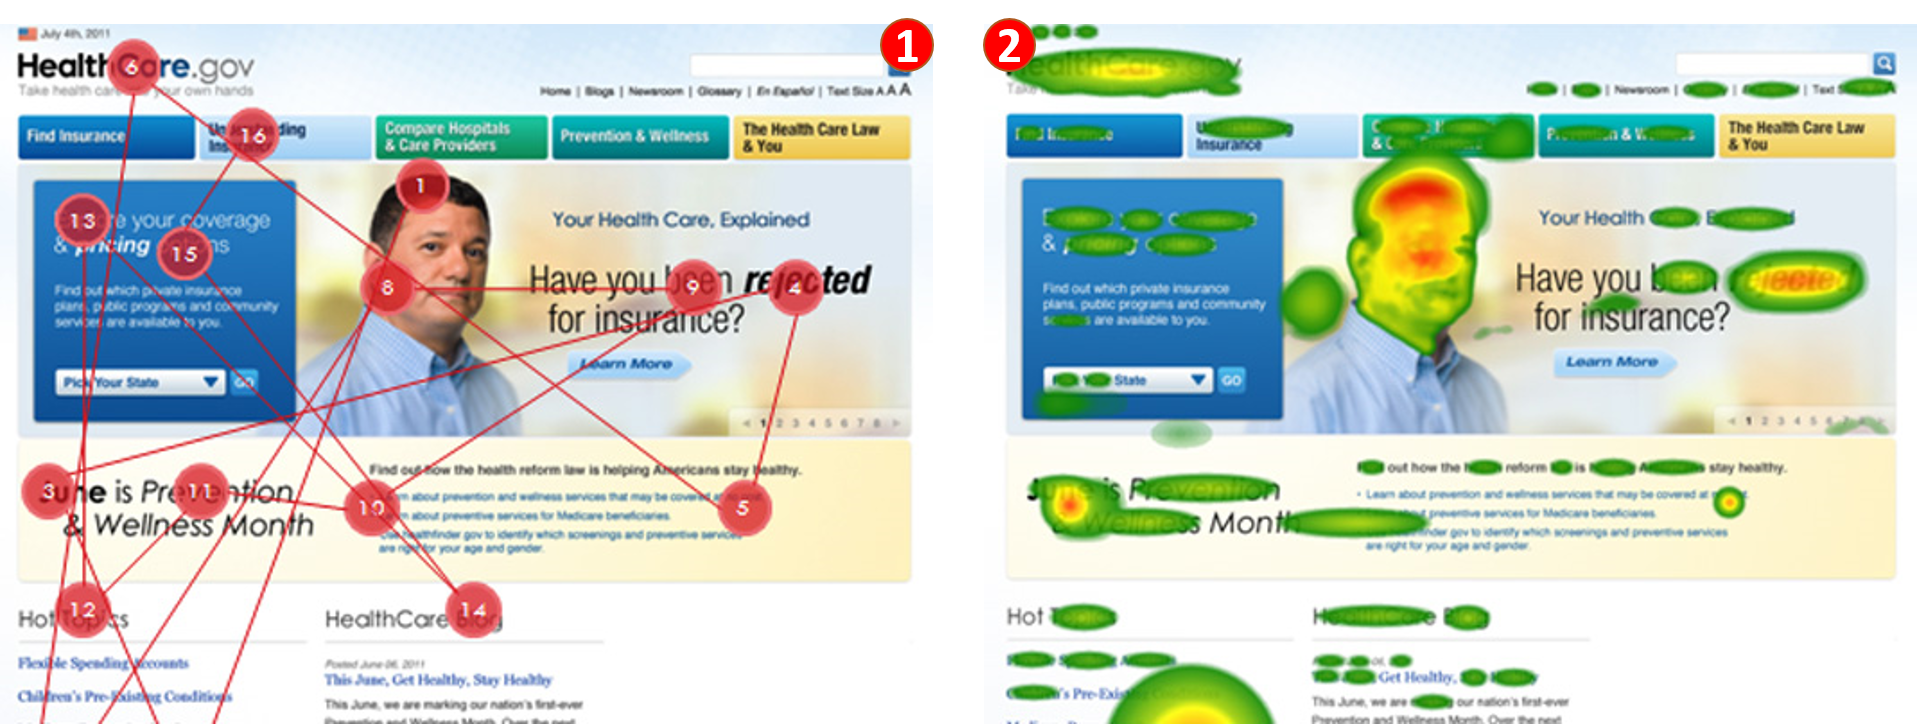
\includegraphics[width=1\linewidth]{img/Evaluation/Eyetracking}
\caption[Auswertungen der Eyetrackinganalyse]{Auswertungen der Eyetrackinganalyse. Linkes Bild (Marker 1): Ansicht einer ausgewerteten Blickabfolge. Rechtes Bild (Marker 2): Ansicht einer ausgewertet Heatmap (Quelle: https://www.usability.gov/how-to-and-tools/methods/eye-tracking.html - Stand Sommer 2016)}
\label{fig:Eyetracking}
\end{figure}


\paragraph{Aufbau des Eyetracking-Test}

\ideas{Beschreibung und Ausarbeitung der Aufgabenstellung -- Sowie die Überlegungen dahinter. Steigender Schwierigkeitsgrad}

Um ein möglichst realistisches Ergebnis der Testes für die Evaluation zu erhalten, orientiert sich der Aufbau weit möglichst an die realen Bedingungen welche im Abschnitt \nameref{Nutzungskontext} beschrieben werden.
Beispielsweise können Abweichung bei der Größe- und Auflösung des Monitors oder des Webbrowsers in dem der Prototyp verwendet wird zu unterschiedlichen Darstellungen führen. 
Dies kann wiederum dazu führen das weniger Informationen angezeigt werden wodurch die Effizienz eingeschränkt wird. (vgl. \cite{Ollermann2007}, S. 40)\\
\\
Für den Test wurde folgende Aufbau verwendet:
\begin{enumerate}
	\item Laptop mit installierter Tobii Software Suite\footnote{Wird verwendet um den Eyetracking Test aufzuzeichnen.}
	\item 24 Zoll Monitor mit einer Auflösung von 1920x1080 Pixel
	\item Mozilla Firefox Version: XXXX
	\item Webcam mit Mikrophon für die Aufzeichnung der Testperson während des Testes
\end{enumerate}

\paragraph{Problemstellung}
Der Test selbst ist in drei Stufen unterteilt, dabei wird bei jeder Stufe die Komplexität zum lösen der Aufgabe erhöht. 
Anhand dieser Vorgehensweise soll anschließend in der Evaluation ermittelt werden, ob wie sich die Bearbeitungsdauer im Vergleich zur Schwierigkeit steigert unter der Berücksichtigung des Erfahrungsgrades der Testperson. 
In jedem der drei Problemstellungen ist die Testperson angehalten eine Außendiensteinsatz zu planen. 
Die jeweilige Schwierigkeit wird dabei durch die zusätzlichen Bedingungen definiert.\\
\\
Als Referenzwert dient der erste Durchgang, hier soll ausschließlich ein Kontakt gefunden und ausgewählt werden. 
In der zweiten Aufgabe wird die Visualisierung von Informationen aus dem System benötigt. Dabei ist wiederum ein Kontakt als primäres Ziel gegeben, die Testperson soll mithilfe des Prototypen sowie den  einem zusätzlichen Auswahlkriterium von der Anweisung weitere Kontakte (sekundäre Ziele) auswählen. 
Im Gegensatz zu den beiden vorangegangenen Aufgaben ist bei der dritten Aufgabe kein Referenzpunkt (primäres Ziel - Kontakt) angegeben. 
Das lösen der Aufgabe besteht darin, eine Menge von potentiellen Zielen auszusuchen, welche den beiden Kriterien aus der Angabe entsprechen.\\
\\
Die Aufgabenstellung welches den Testpersonen ausgehändigt wird befindet sich im Anhang (siehe Abschnitt: \nameref{anhangEyetracking}).


\subsubsection{Fragebogen}
\label{FragebogenEvaluation}


Während beim Eyetracking objektive Messungen  (Dauer des Ablaufs, Blickreihenfolge, etc.) durchgeführt werden stellt die Methode des Fragebogens eine Subjektive Messung da.
Da der Faktor Zufriedenheit in erste Linie subjektiv zu messen ist besteht ein Bedarf dies zu analysieren (vgl. \cite{Ollermann2007}, S. 57).
Zusätzlich besteht die Notwendigkeit, aus Sicht der Evaluierung, weitere Informationen (wie Beispielsweise Selbsteinschätzungen oder Anmerkungen zum Prototypen) ergänzend zum Eyetracking erheben (vgl. \cite{Laugwitz2006}, S. 127). \\
\\
Die Vorteile der Methode des Fragebogens liegen unter anderen in der guten Auswertbarkeit , speziell bei dem Einsatz von geschlossenen Fragen\footnote{Bei geschlossenen Fragen können die Proband\_innen ausschließlich auf vordefinierte Antworten zurückgreifen (vgl. \cite{Ollermann2007}, S. 61)}, der erhobenen Daten was auch der Grund für seine häufige Verwendung (vgl. \cite{Ollermann2007}, S. 61). 
Bei der Erstellung des Fragebogens darauf zu achten, das es sich nicht ausschließlich um eine Ansammlung von Fragen handelt.
Auf der anderen Seite gibt es auch Nachteile, welche unterstreichen das es sich um ein subjektives Verfahren handelt, wie Ollemannn in folgenden vier Punkten skizziert.
Bei dem Halo-Effekt liegt eine Tendenz nahe das die Beurteilung auf Grund eines Globalen Pauschalurteils (Beispielsweise die Farbgebung) gefällt wird.
Die Abgabe von systematisch zu positiven oder negativen Bewertungen (Milde-Härte-Fehler) oder das Gegenteil davon die Zentrale Tendenz bei dem Bewertungen im mittleren Bereich der Skala abgeben werden.
Abschließend führt er den Primacy-Recency-Effekt auf bei der die Bewertung durch die Reihenfolge der einzelnen Fragen beeinträchtigt wird. (siehe \cite{Ollermann2007}, S. 60)\\
\\
Damit der Fragebogen als funktionales Werkzeug bei der Evaluierung eingesetzt werden kann empfiehlt Burmester zusätzlich die Beachtung von Gütekriterien bei der Erstellung. 
Dabei handelt es sich sind unter anderen um das Gütekriterium der Validität\footnote{Der Fragebogen sollte darauf ausgelegt sein, dass zu messen was er vorgibt. (nach \cite{Burmester}, S. 350)}, - das Gütekriterium der Reliabilität\footnote{Ein wiederholtes Durchführen, unter den gleichen Bedingungen, soll zu dem selben Ergebnis führen. (nach \cite{Burmester}, S. 350)} und das Gütekriterium der Objektivität\footnote{Das Ergebnis ist unabhängig von der Person, welche die Untersuchung durchführt. (nach \cite{Burmester}, S. 350)}. \\
\\
\begin{comment}
Aufbau des Fragebogens
\end{comment}
Neben der Erfragung der subjektiven Meinung über das Produkt soll nach Ollermann auch Informationen über den Hintergrund der befragten Person erhoben werden.
Um diesen Hintergrund zu protokollieren empfiehlt er folgende Aspekte zu erheben Alter, Geschlecht und Erfahrung.
Speziell der Grad der Erfahrung stellt laut Ollermann einen "wesentlichen Einflussfaktor" für die Gebrauchstauglichkeit da. (vgl. \cite{Ollermann2007}, S. 46). 
Neben der eigentlichen Erfahrung mit dem Umgang von Pery, in welches der Prototyp eingebettet ist, stellt sich auch vergleichsweise die Frage ob und wie ausgeprägt Erfahrungen mit den Webservices vorhanden sind welche im Kapitel \nameref{chap:analyse} behandelt werden (siehe Abschnitt: \nameref{chap:analyse:sec:sota:sec:google_maps}, \nameref{Airbnb} und \nameref{Flightradar}).
\\
\\
In erster Linie dient der Fragebogen, wie Eingangs erwähnt, als Unterstützung für die \nameref{Eyetracking}-Tests um eine subjektive Meinung bezüglich der drei Gebrauchstauglichkeits-Dimensionen zu erheben. 
Zum einen basiert der Fragebogen aus eigenen Fragen zum anderen in Anlehnung an standardisierten Fragebögen.
Von den standardisierten Fragebögen handelt es sich zum einen um den Fragebogen IsoMetric S (vgl. \cite{IsoMetricS}) und zum anderen um ISONORM (vgl. \cite{IsonormL}).
Da der ISONORM Fragebogen für die Analyse der Software Ergonomie-Norm (vgl. \cite{IsonormL}, S. 1) und nicht der Gebrauchstauglichkeit werden nur wenige Fragen erstellt die auf diesem Fragebogen basieren.
Im Gegensatz dazu, dient der IsoMetrics-Fragebogen als weitaus größere Kreativitätsquelle bei der Erstellung des Fragebogens.
Speziell die Möglichkeit, das Testpersonen sich bei Fragen ihrer Bewertung enthalten können wird als nützliches Element in die Befragung aufgenommen\footnote{Vorbeugung des Zentrale Tendenz-Problem welches zuvor in diesem Abschnitt beschrieben wurde.}\\
\\
Zusätzlich ist am Ende des Fragebogens/Interviews Platz für Anmerkungen vorgesehen welche während des Eyetrackings von den Testpersonen geäußert wurden.
An dieser Stelle soll mithilfe der entsprechenden Testperson geklärt werden wodurch diese Aussage provoziert wurde und ob sie negativ oder positiver Natur ist. (vgl. \cite{Niegemann2008}, S. 422)\\
\\
Der finale Fragebogen kann im Anhang (siehe Abschnitt: \nameref{anhangFragebogen}) eingesehen werden.


\subsection{Stichprobenbeschreibung}
\label{Stichproben}
In Summe wurde die Evaluation mit elf Personen durchgeführt. 
Dabei lag der mittlere Wert des Alters bei 25,5 Jahren (min: 22 Jahren, max: 29 Jahren, einmal keine Angabe). 
Die elf Personen gaben dabei folgende Nennungen beim Geschlecht an: dreimal männlich, sechsmal weiblich sowie zweimal kein Angabe.
Da der Prototyp als Erweiterung für Pery implementiert ist werden die Testpersonen, anhand Ihrer Erfahrungen im Umgang mit Pery, in drei Gruppen eingeteilt. 
Dabei wurden die Gruppen wie folgt definiert: 
\begin{itemize}		
	\item Gruppe 1: keine Erfahrung mit Pery 
	\item Gruppe 2: geringe bis mittlere Erfahrung mit Pery
	\item Gruppe 3: ausgeprägte Erfahrung mit Pery
\end{itemize}
Die Zuordnung der Testpersonen zu denn entsprechenden Gruppen wurde anhand der Faktoren der durchschnittliche Verwendung von Pery (in Stunden pro Woche) sowie der Dauer (in Monaten) seit dem Pery in Verwendung ist durchgeführt.
Anhand dieser Zuordnung ergab sich das sechs Personen der Gruppe 1, drei Personen der Gruppe 2 und zwei Personen der Gruppe 3 zugeordnet werden. 

\section{Ergebnisse}
\label{Ergebnisse}
\ideas{nüchtern und ohne Interpretation}
Die Evaluation bestand aus den drei Teilen Einführung, Eyetracking und Interview. 
Dabei variierte der Einführungsteil je nach Hintergrund und Vorwissen der Person. 

\section{Interpretation \& Diskussion}
\label{InterpretationDiskussion}



\end{document}